\chapter{Receiving OSNMA: First Steps}
\label{ch:osnma_first_steps}

In the next two chapters we'll take a critical look at the OSNMA specification,
trying to reformulate it from a receiver point of view. The goal is to identify
key areas of possible improvement for the protocol, together with critical
aspects for a receiver implementation, and to provide suggestions for both.
We'll start with analysing what it takes for a new receiver to be able to
authenticate the navigation message.

\vspace{\baselineskip}

When thinking about a Galileo receiver capable of supporting OSNMA, we can
identify two distinct modes of operations: a bootstrap phase and a nominal one.
In the bootstrap phase the receiver doesn't possess any data apart from a public
key capable of authenticating a DSM; therefore in this phase the receiver is not
formally capable of authenticating the navigation message, and needs to perform
operations which can bring it into the nominal mode. In this phase the receiver
is capable of authenticating the navigation message using the data it has stored
locally and the MACK sections it receives together with the unauthenticated
message.

This distinction is purely analytical in nature, but can help breaking down the
problem into distinct blocks, which will be separately analyzed in the chapters
to follow.

\vspace{\baselineskip}

For the bootstrap phase we'll consider a generic Galileo receiver with no access
to any data network other than the radio channels over which the Galileo
satellites transmit. This receiver has never received any navigation
data before, and only contains onboard a set of public keys that should allow it to
verify the authenticity of the root keys sent in the DSM-KROOT section.

To keep the discussion focused, we'll skip over the specific details of
acquiring one or more signals and we'll assume the receiver can enter the
acquisition phase for a sufficient number of in-view satellites, and to
successfully move into the tracking phase which will allow it to decode the
Galileo navigation data frame.

\vspace{\baselineskip}

Under these conditions, when the receiver starts its operations it has no
knowledge about the key chain currently in force, and therefore if it wants to
authenticate the navigation message the first thing it has to do is to receive a
DSM-KROOT and decode the root key. We'll start our analysis from here.

\section{Root key authentication}
The root key is sent in the HKROOT section of the navigation data frame. This
section of data is transmitted at a rate of 8 bits every 2s (i.e. 4bps) and is
composed of two headers of 8 bits each, and of a variable number of blocks of
104 bits. Each subframe contains the two headers and a DSM block. According to
the current specification, the number of blocks that compose a DSM can vary
between 6 and 16 (but there are 5 reserved values so it could possibly be
longer). In order for a receiver to be able to correctly compose a DSM, in the
first block the total number of blocks is sent.

\subsection{HKROOT receiving time}
The first simple conclusion we draw from what we've seen so far is that
reception of a whole DSM takes between 180s and 480s. In order to speed up the
bootstrap operation a receiver might cache the navigation message sent, provided
it won't use it until it has been authenticated in full. The amount of caching
memory needed will be analyzed later on in the chapter.

\subsection{Variable size of the DSM}
A second observation is about not knowing the precise size of the DSM upfront.
Since the receiver needs to cache the DSM until it's fully received and can be
decoded, two general approaches are possible:
\begin{enumerate}
  \item a fixed amount of memory is allocated that accounts for the longest
    possible DSM. This memory could be separate from the RAM associated with the
    CPU that perform the authentication operations, in order to avoid security
    problems due to buffer overflows. This could be expensive and inefficient
    (for example, if a DSM is only 6 blocks long, then the memory reserved for
    the other 10 blocks is wasted)
  \item the RAM of the computational unit is used to cache the DSM until it's
    possible to decode it. In this case, a variable amount of memory is
    allocated, and two strategies could be followed to manage the length
    variability:
    \begin{enumerate}
      \item the receiver makes sure that it starts decoding a DSM from its first
        block, which contains the information about the total number of blocks.
        This means potentially discarding several minutes of data
      \item the receiver stores the blocks as individual pieces of information
        and then recombines them at the end (for example, using some form of
        sorting algorithm), or on the fly (for example, using something like a
        linked list)
    \end{enumerate}
\end{enumerate}

This scenario offers the possibility for several considerations. The first one
is that, no matter the strategy chosen to store the DSM blocks, care must be
taken not to expose the receiver to memory overflow attacks. Since the data
that's being received at this point in time is not authenticated yet, it could
also be forged by an attacker who would send more blocks than what stated
in the first DSM block. If a receiver doesn't implement a preventive check, this
kind of attack might allow an attacker to overwrite some reserved memory with
executable malicious code. A simple check that the number of the block being
processed is within the advertised length is sufficient to prevent this kind of
vulnerability.

The second consideration is that neither of the scenarios in option 2) are ideal.
In fact option 1) is safer, but results in even longer bootstrap times. The
second option is faster but it's based on the assumption that the satellites
will keep sending the same key over and over again (i.e. if blocks with lower
indexes are missed, then they can be received later on by a subsequent
transmission of the same key). Moreover, dealing with the unknown length of the
DSM requires more expensive data structures and operations.

That said, an ideal approach for a receiver would be to learn the total length
of the DSM no matter at what point of its transmission it starts to receive.
This way the receiver could allocate all the needed memory at once, and
subsequently fill in the gaps with the received blocks (provided it also
implements the check to prevent memory overflow attacks). In the OSNMA protocol
this could be achieved by sending the field \textit{Number of blocks} in the DSM
header rather than the first block of the DSM. This would increase the size of
the DSM Header from 8 bits to 12 bits, resulting in an additional overhead that
ranges between 24 bit (when a DSM is composed of 6 blocks) to 64 bits (when a
DSM is composed of 16 blocks).

\section{Initial key authentication}
The specification provided in \cite{osnma} recommends for a single key chain
an extension of $2^{25}$ to $2^{26}$ keys. The actual duration of such a chain
is dependent on the key size, the number of satellites and the number of MACK
sections per subframe; with a key size of 82 bits, 36 satellites and 3 MACK
sections per subframe, the chain would have a duration of about 4 months.

Under these assumptions, we can try to analyze the scenario in which a receiver
with no prior navigation data starts to receive a navigation message inclusive
of DSM and verification tags, and subsequently tries to authenticate the
received key against the root key of the chain.

One hypothesis we make to analyze this scenario is that the key included in the
DSM-KROOT section is the key with index $0$. That is, the constellation doesn't
authenticate any other, more recent, key. This clarification is necessary since
the protocol specification declares the possibility of transmitting more recent
keys (i.e. with index higher than $0$) in the DSM, but doesn't provide any
detail on how that would work. To separate the two problems, we provide here a
worst-case analysis that's independent from the transmission of floating KROOTs.

\subsection{Receiver operation}

Having laid out the context, we can proceed to describe the set of operations
a receiver is required to perform in order to authenticate the navigation
message.

Let's assume the receiver already received and decoded a sufficient amount of
data to calculate the pseudorange against a satellite and to authenticate
mentioned data. This includes having at hand at least one MAC $t_m$, the key that
has been used to produce it $K_m$, and the root key $K_0$.

Given only this set of data, in order to authenticate the key $K_m$ the
receiver must perform precisely $m$ invocations of the one-way hashing function
$F$ in order to verify that $K_0 = F^m(K_m)$. At the end of the calculation, the
receiver will obtain $K_0' = F^m(K_m)$; if $K_0' = K_0$ (i.e. the calculated key
matches the one embedded in the DSM), then the authentication of $K_m$ is
successful. Otherwise, the key and associated data must be discarded.

We can then easily see that if a receiver starts to receive data at the end of a
key chain of length $L+1$, the initial key authentication will require applying
$L$ times the hash function to $K_L$.

\subsection{Initial authentication benchmarking}

Following this result, we perform a benchmark to understand time and
resource consumption to aid hardware design and implementation for receivers
that should support OSNMA.

The algorithm described so far contains three degrees of freedom that have been
analyzed separately: chain length, key length and selected hash function. As
stated, the recommended chain length is between $2^{25}$ and $2^{26}$; to
provide a more extensive overview our benchmark ranges between $2^{20}$ and
$2^{30}$ keys. The options for key length are fixed and provided in the
\textit{Key Size} included in the DSM-KROOT; these range between $80$ and $256$.
The possible hash functions are SHA256, SHA3-224 and SHA3-256.

Given the limited availability of open source libraries that support SHA3 at the
time of writing, we've chosen to perform the benchmarking using \textbf{Python
3.6}. Since this dynamic language is not what usually gets used to write
embedded code, we've compared its performances with a C implementation of the
same logic. The two programs both measure the time it takes to perform $2^{20}$
computations of a SHA256 chain.

\vspace{\baselineskip}

The first test measures how much time it takes to compute the whole chain of
keys, for different lengths of the chain. Tested lengths vary between $2^{20}$
and $2^{30}$ keys, so that the suggested values of $2^{25}$ and $2^{26}$ lie in
the middle of the range. The computation is done against a fixed key of $80$
bits of length, and the same test has been performed for all the hash functions
supported by the protocol.

\begin{figure}[h!]
  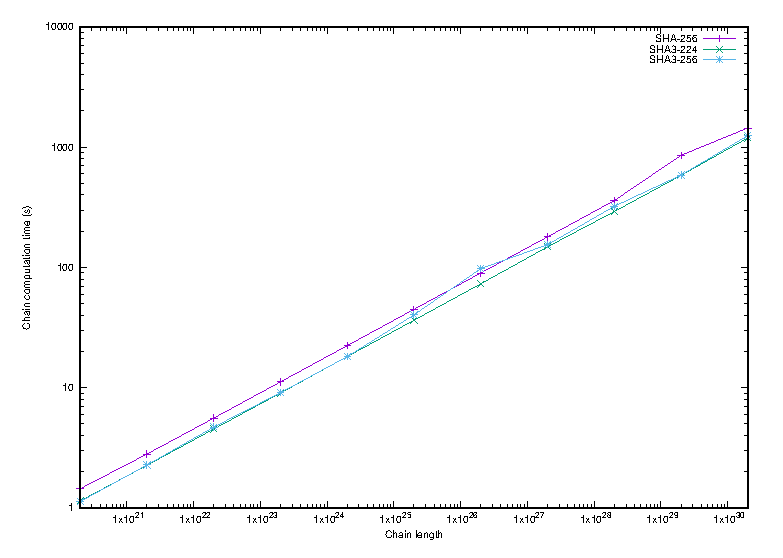
\includegraphics[width=\linewidth]{figures/chain_speed.eps}
  \caption{Chaing length vs computation time of the whole chain}
  \label{fig:bm1}
\end{figure}

The results of this first benchmark can be seen in figure~\ref{fig:bm1}. The values
that make up the graph can be seen in table~\ref{table:bm1}. It's important to
observe that the both axis are in logarithmic scale.  We can observe
that the relationship is basically linear with little difference between hash
functions: that is, no matter the function chosen, doubling the size of the
chain directly doubles the time it takes to compute the chain.

\begin{longtable}[]{@{}llll@{}}
\toprule
Chain size & SHA-256 & SHA3-224 & SHA3-256\tabularnewline
\midrule
\endhead
$2^{20}$ & 1.4449 & 1.1455 & 1.1296\tabularnewline
$2^{21}$ & 2.8077 & 2.2665 & 2.2768\tabularnewline
$2^{22}$ & 5.5871 & 4.5320 & 4.7067\tabularnewline
$2^{23}$ & 11.189 & 9.0380 & 9.0916\tabularnewline
$2^{24}$ & 22.408 & 18.161 & 18.170\tabularnewline
$2^{25}$ & 44.857 & 36.362 & 40.316\tabularnewline
$2^{26}$ & 89.838 & 73.052 & 97.746\tabularnewline
$2^{27}$ & 179.45 & 148.20 & 154.51\tabularnewline
$2^{28}$ & 359.15 & 291.50 & 321.99\tabularnewline
$2^{29}$ & 855.27 & 582.81 & 586.11\tabularnewline
$2^{30}$ & 1442.6 & 1192.6 & 1247.0\tabularnewline
\bottomrule
\caption{Key chain computation time [s] vs key chain length}
\label{table:bm1}
\end{longtable}

Another general observation is that the computation time improves slightly for
the SHA3 family of hash functions, but in general the variability in computation
time is dominated by the chain length.

One important aspect to focus our attention on is the relative significance of
this benchmark with respect to the average computation power of a common 
receiver. The numbers just described have been obtained by running the code on a
MacBook Pro sporting a 2.6GHz Intel Core i5 processor. A benchmark sheet such as
\cite{bm_intel_core_i5} can show that such a processor can handle roughly $50
000$ DMIPS. As a reference, the STA8088EXG GNSS receiver \cite{st_rec_specs}
sports an ARM9 processor clocking at a maximum of 208MHz. Usually in such
receivers the CPU clocks at much lower rates than their maximum (see for example
\cite{mediatek_specs}). According to the ARM Information Center website
\cite{armkb}, the maximum performance of the ARM9 family reaches $1.1$ DMIPS per
MHz, which means we can assume the reference CPU can achieve roughly $230$ DMIPS
when at full speed.

In order to translate these observations to an estimate of the running time for the
chain computation on an embedded device, we've correlated the running time of
the Python code to that of its C counterpart. Surprisingly, the same benchmark
for a key chain of length $2^{20}$ over the SHA-256 function seems to perform
better in Python than in C, as exposed in table~\ref{table:bm_c_python}. As a
reference, the Python snippet is provided in listing~\ref{lst:python_bm} and its
C counterpart in listing~\ref{lst:c_bm}. This is because the Python
implementation uses the same libraries as the C code, but the Python environment
calls out to architecture-specific assembly implementations of those functions.
In any case, this shows that the performances of the two implementations are
within the same order of magnitude, so comparing directly against the Python
results is a good approximation of the best case scenario.

\lstinputlisting[
  language=python,
  caption={Computing $2^{20}$ SHA256 hashes in Python 3.6},
  label={lst:python_bm}
]{code/bm_initial_auth.py}

\lstinputlisting[
  language=c,
  caption={Computing $2^{20}$ SHA256 hashes in C},
  label={lst:c_bm}
]{code/bm.c}

\begin{longtable}[]{@{}ll@{}}
\toprule
Python & C\tabularnewline
\midrule
\endhead
1.4449s & 2.2960s\tabularnewline
\bottomrule
\caption{Average computation time for the calculation of $2^{20}$ SHA256 hashes
in Python vs C}
\label{table:bm_c_python}
\end{longtable}

In other words, this comparison tells us that in order to get an estimate of how
long it would take to compute the whole key chain on an embedded CPU of a
Galileo receiver we can simply relate the running times $t_j$ just measured, the
processing power of the CPU where the benchmark was run $P_{BM}$ and the
projected processing power of the CPU of the receiver $P_R$. The processing
power is measured in DMIPS, a definition of which can be found in \cite{dmips}.
A simple proportion shows that

\begin{equation}
  t_j / P_{BM} = t_{rj} / P_R
\end{equation}

where $t_{rj}$ is the estimate of the running time on the receiver processor. This
equation solved for this last variable yields:

\[
  t_{rj} = t_j \frac{P_{BM}}{P_R}
\]

Substituting the variables with the numbers devised above we can obtain an
approximate conversion as follows:

\begin{equation}
  \label{eq:mips_conv}
  \begin{aligned}
  t_{rj} &= \frac{50 \cdot 10^3}{230} t_j\
        = 246.30 t_j
  \end{aligned}
\end{equation}

Applying this conversion rate to table~\ref{table:bm1} we obtain the numbers in
table~\ref{table:bm1_recv}.

\begin{longtable}[]{@{}llll@{}}
\toprule
Chain size & SHA-256 & SHA3-224 & SHA3-256\tabularnewline
\midrule
\endhead
$2^{20}$ & 355.88 & 282.14 & 278.22\tabularnewline
$2^{21}$ & 691.54 & 558.24 & 560.78\tabularnewline
$2^{22}$ & 1376.1 & 1116.2 & 1159.3\tabularnewline
$2^{23}$ & 2755.9 & 2226.1 & 2239.3\tabularnewline
$2^{24}$ & 5519.1 & 4473.1 & 4475.3\tabularnewline
$2^{25}$ & 1.1048e4 & 8956.0 & 9929.8\tabularnewline
$2^{26}$ & 2.2127e4 & 1.7793e4 & 2.4075e4\tabularnewline
$2^{27}$ & 4.4199e4 & 3.6502e4 & 3.8056e4\tabularnewline
$2^{28}$ & 8.8459e4 & 7.1796e4 & 7.9306e4\tabularnewline
$2^{29}$ & 2.1065e5 & 1.4355e5 & 1.4436e5\tabularnewline
$2^{30}$ & 3.5531e5 & 2.9374e5 & 3.0714e5\tabularnewline
\bottomrule
\caption{Approximate key chain computation time [s] vs key chain length for an
average GNSS receiver}
\label{table:bm1_recv}
\end{longtable}

By looking at this result we can see how the worst case scenario might result
in severe energy consumption by the receiver itself. Considering just the
lengths that have been proposed in the specifications, we can see how a receiver
might spend between 3.5 and 5 hours of computation just to perform the
authentication of a single key. Considering the case of mobile devices such as
smartphones, this is an amount of time that can have a noticeable negative
impact on battery level and might make data authentication infeasible for common
uses.

To complete the analysis, we evaluated the change in computation time as
the key length varies. As figure~\ref{fig:key_length} shows, there's a slight
increase in computation time of a single hash in the case of SHA-256 when the
key size reaches around 180 bits, but in the case of the other functions the
computation time remains constant. This leads to the conclusion that computation
time is bound only by the length of the chain, and all other parameters don't
affect the receiver in a significant way.

\begin{figure}[h!]
  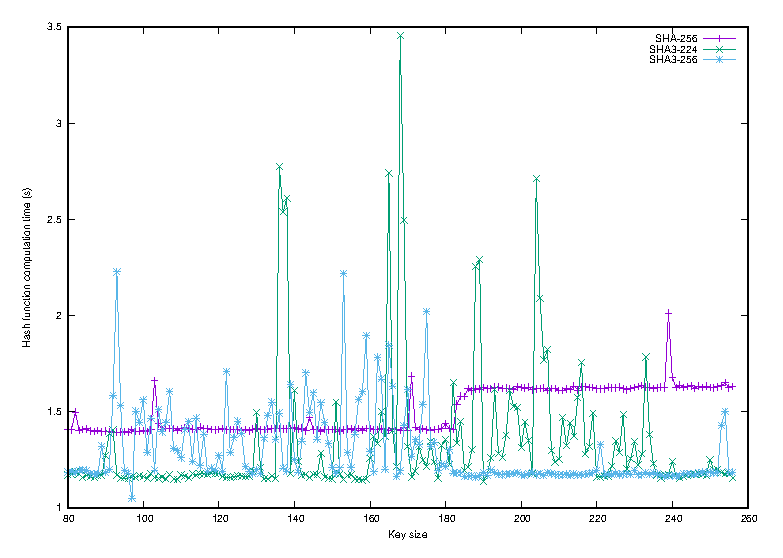
\includegraphics[width=\linewidth]{figures/key_length.eps}
  \caption{Key length vs computation time of the supported hash functions}
  \label{fig:key_length}
\end{figure}

\section{Floating KROOTs}
As part of the protocol specification described in \cite{osnma}, a mention
is made regarding the possibility of sending DSM for KROOTs other than the one
with index $0$, but no further information related to how this would work are
provided. In this section we dwelve deeper into the topic and make some hypothesis
on how floating KROOTs could be managed effectively and efficiently.

Due to the nature of the key chain in TESLA, a key $K_m$ sent as part of a MACK
section can be authenticated against any other key $K_j$ with index $j < m$ that
has already been authenticated by the receiver. The only condition for this to
work is to know how many times the receiver needs to invoke the hashing function
$F$ over the key $K_m$ in order to obtain $K_j$.

Unfortunately OSNMA doesn't send explicit key indices, but being the navigation
message sent at a fixed bit rate, the time of transmission of a subframe can
be used to identify a key in the chain. In order to calculate the distance
between the two keys, a receiver needs to consider:
\begin{itemize}
  \item $t_m$: the time (in seconds) of transmission start of the subframe in
    which $K_m$ is applied
  \item $t_j$: the KROOT time (in seconds) calculated as combination of KROOT WN
    and KROOT DOW as described below
  \item $n_M$: the number of MACK sections contained in a subframe, as sent in
    the \textrm{NMACK} field in the HKROOT section. This directly relates to the
    number of keys applied in a subframe as one MACK section always contains one
    key
  \item $p$: the relative position of key $K_m$ in the chain starting from the
    first key of the first MACK section of the subframe in which $K_m$ is sent
  \item $NS$: the number of satellites, normally set to 36 as per protocol
    specification
\end{itemize}
Once these parameters are known, then it's possible to calculate the distance
between the keys as follows:
\begin{equation}
  \label{eq:d}
  d = \frac{t_m - t_j}{30} n_M \cdot \textrm{NS} + p
\end{equation}

In plain words, this equation means that the number of keys in the chain between
the root key and the key being received is composed of the sum of the number of
keys used to authenticate all the previous subframes for all satellites and the
number of keys that stand in between the received key and the first key in the
subframe that's currently being read by the receiver.
Having decomposed this result in these two parts we can now analyze how to
calculate $t_m - t_j$ and $p$, since OSNMA doesn't send these parameters
explicitly.

To calculate $t_j$, we can start from the week number \textrm{KROOT WN} and the
day of week \textrm{KROOT DOW} associated to the KROOT that are sent in the
HKROOT section. These two parameters identify the KROOT in the following way:
the KROOT is the key immediately preceding the key in the chain whose
application time coincides with a subframe being sent at the beginning of the
day of week in the week number just mentioned.

From this, we can derive that
\begin{equation}
  \label{eq:t_j}
  t_j = t_0 + \textrm{WN}_j \cdot 604800 + \textrm{DOW}_j \cdot 86400
\end{equation}
where $t_0$ is the GST epoch time, $604800$ is the number of seconds in a week
and 86400 is the number of seconds in a day.

With the same line of reasoning, we can calculate $t_m$ by using the GST of the
start of the subframe in which $K_m$ is sent. According to \cite{galileoicd},
this is composed of two fields: the week number counted from the GST epoch, and
the time of week $\textrm{TOW}$ in seconds; this yields:
\begin{equation}
  \label{eq:t_m}
  t_m = t_0 + \textrm{WN}_m \cdot 604800 + \textrm{TOW}_m
\end{equation}

Now expanding ~\ref{eq:t_j} and ~\ref{eq:t_m} in ~\ref{eq:d} we obtain:
\begin{equation}
  \label{eq:d2}
  \begin{aligned}
    d &= \frac{(t_0 + \textrm{WN}_m \cdot 604800 + \textrm{TOW}_m) - (t_0 +
    \textrm{WN}_j \cdot 604800 + \textrm{DOW}_j \cdot 86400)}{30} n_M \cdot
    \textrm{NS} + p \\
    &= \frac{\textrm{WN}_m \cdot 604800 + \textrm{TOW}_m - \textrm{WN}_j \cdot
    604800 - \textrm{DOW}_j \cdot 86400}{30} n_M \cdot \textrm{NS} + p \\
    &= \frac{(\textrm{WN}_m - \textrm{WN}_j) \cdot 604800 + (\textrm{TOW}_m -
    \textrm{DOW}_j \cdot 86400)}{30} n_M \cdot \textrm{NS} + p
  \end{aligned}
\end{equation}

What remains to be done now it so calculate the parameter $p$. In order to do
so we need to keep again into consideration the fact that the keys belonging
to a single key chain are spread across satellites and that therefore
consecutive keys in MACK sections sent from the same satellite are actually
separated by $\textrm{NS}$ keys. In addition to that, since there is no index
sent within the MACK sections, the receiver needs to keep a counter $l$ of how
many keys it receives within a subframe (this counter will be reset with every
new subframe). This will directly count the position of a given key within the
sub-chain starting at the beginning of the subframe. This allows us to define
$p$ as
\begin{equation}
  \label{eq:p}
  p = l \cdot \textrm{NS}
\end{equation}

Finally, expanding ~\ref{eq:p} into ~\ref{eq:d2} we obtain:
\begin{equation}
  \begin{aligned}
    d &= \frac{(\textrm{WN}_m - \textrm{WN}_j) \cdot 604800 + (\textrm{TOW}_m -
    \textrm{DOW}_j \cdot 86400)}{30} n_M \cdot \textrm{NS} + l \cdot \textrm{NS} \\
    &= \left[\frac{(\textrm{WN}_m - \textrm{WN}_j) \cdot 604800 + (\textrm{TOW}_m -
    \textrm{DOW}_j \cdot 86400)}{30} n_M  + l\right] \cdot \textrm{NS}
  \end{aligned}
\end{equation}

A first observation we can make regarding this result is that calculating the
distance between two keys is not as straightforward as it could be for an
embedded receiver. While it's true that it involves only integer arithmetic, it
still requires the receiver to perform multiplications and divisions. This is
true also for calculating the distance between two random keys in the chain, not
just between a key in a MACK section and a root key. While the complexity of
this calculation is not as high as that described above to correlate a key at
the end of the chain with the root key, it is nevertheless an operation that
needs to be run often, as every received key needs to be correlated to a
previously authenticated key by means of its distance to it. A possible
optimization could be to send an index along with the keys (both in the floating
KROOT and MACK sections). This would not only reduce the receiver operations to
just one single subtraction, but also make the key generation strategy
transparent to the receiver (i.e. if the ground segment decides to change the
way keys are spread across satellites, there would be no need to reprogram the
receivers).

A second observation is that the time resolution for floating KROOT is 1
day. This means that not every key can be used as a floating KROOT, but rather
only the first key that is applied at the beginning of a Galileo day can be
correctly targeted by means of the KROOT WN and KROOT DOW parameters. This means
that approximately 1 out of a minimum of ~103680 and 1 out of a maximum of
~414720 keys can be used as floating KROOTs \footnote{these two numbers are the number of
keys sent in a day in the case where either 1 or 4 keys are consumed in a
subframe, calculated by multiplying the number of keys in a subframe by the
number of satellites and by the number of subframes in a day:
$\frac{86400}{30}36 \cdot \textrm{NMACK}$}.

If we make the assumption that a new floating KROOT is broadcast and signed
every day, we can then consider this result in a similar fashion as done above
for the first KROOT. In particular, we can consider the number of keys sent in a
day as being the maximum distance that keys will have from the nearest KROOT,
and this in turn allows us to derive a loose upper bound on how long it can take
under these circumstances to verify a key against a floating KROOT. Applying the
same benchmark script as used in the previous section, and applying the same
performance conversion devised in ~\ref{eq:mips_conv}, we obtain the numbers in
table ~\ref{table:float_kroot}.

\begin{longtable}[]{@{}lll@{}}
\toprule
  Distance from KROOT & Time on Intel Core i5 (s) & Est. time on ARM (s)
  \tabularnewline
\midrule
\endhead
  103680 & 0.1411 & 34.753 \tabularnewline
  414720 & 0.5688 & 140.10 \tabularnewline
\bottomrule
  \caption{Upper bounds for authentication of a key against a floating KROOT}
\label{table:float_kroot}
\end{longtable}

This is a definite improvement over the time it takes to authenticate a key at
the end of the chain with the root key at its beginning, but depending on the
receiver computational capabilities it might still be an expensive operation to
perform.

% MAYBE if you have time
% Conclusions:
% - proposal on the frequency of floating KROOT
% - based on that, proposal on reducing the overall length of the chains and
%   eliminating the need for floating KROOTs -> maybe not, as keeping the chain
%   long might allow long-lived receivers to keep authenticating keys in the
%   chain without the need of receiving new KROOTs

\section{Clock synchronization}

\subsection{TESLA security condition in OSNMA}

One of the prerequisites of TESLA is for the clocks of receiver and sender to be
loosely synchronized. More specifically, TESLA is based on a security condition
that allows the receiver to identify a packet arrived safely by knowing
unambiguously that the corresponding key disclosure packet has not been
transmitted yet. This is because, should the opposite hold true, an attacker
could have received the key disclosure packet and forged a message using that
key; without the guarantee specified in the security condition the receiver has
no way to detect this kind of attack.

In OSNMA it's still necessary to meet this condition in order to guarantee the
security of the whole algorithm. We'll describe next a possible attack that
relies on the clock of the receiver being undefinitely out of sync with system
time.

\subsection{An attack against clock synchronization}
The scenario is composed of the following actors:
\begin{itemize}
  \item a legitimate Galileo satellite, sending authenticated navigation data
    following the OSNMA specification. The clock of this sender is perfectly
    synchronized with the central system time
  \item a Galileo receiver with an unknown clock drift $\delta_t$ upper bounded
    by a known fixed value $\delta_{max}$
  \item an attacker capable of receiving Galileo navigation data and transmit a
    custom signal resembling that of one or more Galileo satellites, and
    containing ad-hoc forged data.
\end{itemize}

In this scenario the attacker is free to modify the received data, but is
limited in the following:
\begin{itemize}
  \item it cannot forge the root key transmitted in the HKROOT section. This is
    based on the security of the asymmetric scheme used to authenticate the root
    key
  \item for the same reason, it cannot forge the transmission time of mentioned
    key. The transmission time (in form of the Galileo week number and day of
    week) is included in the signature and such forgery would be detected with
    the same high probability as a forged key
  \item if it wishes to reuse a key of the chain, it must send it in the right
    order with respect to the others and with the right time. This is because
    the transmission time of a key univocally determines its index in the chain,
    and the transmission time is also authenticated in the MACs sent in the
    MACK sections. Should the key be sent out of order (i.e. with the wrong
    time), the receiver wouldn't be able to authenticate it against the root key
\end{itemize}

Another assumption we make is that the receiver is already sending a forged
navigation message before the receiver starts to receive on the same frequency
the attacker is transmitting. The message sent by the attacker contains a forged
set of ephemeris crafted so that the receiver would derive a set of coordinates
different than its real ones. This data is authenticated using the OSNMA
protocol as follows:
\begin{itemize}
  \item the attacker receives the legitimate signal at time $t_k$, reading the
    keys contained in the MACK sections
  \item the attacker uses the keys it read in the same orders as they were
    received to authenticate the forged data
  \item the forged data is transmitted at time $t_k + \delta_f$ with a power
    sufficient to spoof the legitimate signal
\end{itemize}

Here $\delta_f$ is a delay that accounts for the fact that a key is necessarily
read after the corresponding MACs, but the attacker needs to replace the MACs
\textit{after} having read the key, so the resulting message needs to be delayed
by a fixed amount of time that allows the attacker to perform the attack and
build a valid navigation message.

\begin{figure}[h!]
  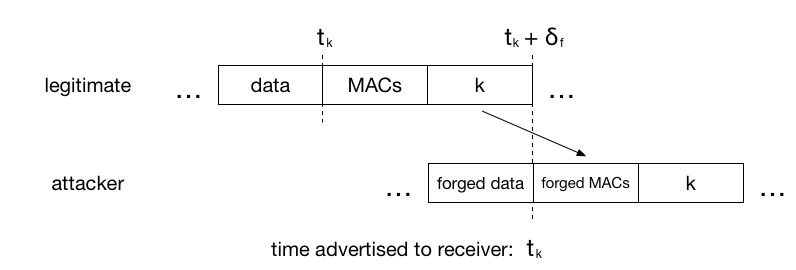
\includegraphics[width=\linewidth]{figures/delay_attack.png}
  \caption{Possible forging attack that relies on lack of clock synchronization}
  \label{fig:delay_attack}
\end{figure}

Under these conditions we can see what happens on the receiver side:
\begin{itemize}
  \item When it wakes up, the receiver immediately starts to acquire and track
    the forged signal. Since its clock offers no guarantees of synchronization
    against system time, the receiver is not capable of spotting that the
    received signal is delayed.
  \item At first the receiver will decode and authenticate the root key; this
    operation will succeed since the attacker is just sending a delayed version
    of the original data.
  \item Once the root key is authenticated, the receiver starts to receive the
    navigation message and the respective MACK sections. The receiver at some
    point will verify that the GST advertised in the subframe matches 
    the time that has been signed by the keys it's receiveing; this operation
    will also succeed since at this point the receiver has no knowledge of the
    true system time and the attacker is correctly building the signatures
    following the protocol.
  \item The receiver will proceed by authenticating the key it received against
    the root key. This step will also be successful as no forgery is necessary
    on the time parameters of the navigation message, and the order of the keys
    is being preserved by the attacker.
\end{itemize}

As shown by the above example, without guarantee of synchronization between the receiver
and sender's clocks, and without an upper bound on the drift between the two, a
spoofing attack can go undetected even in the presence of data authentication in
case a receiver starts receiving without prior knowledge of any system
parameter. We'll describe next how this risk could be mitigated.

\subsection{Preventing forgery attacks}
The problem just described is addressed in \cite{perrig} as a prerequisite to
the algorithm: i.e. TESLA doesn't provide any mechanism to synchronize
the clocks beforehand, but rather demands that an upper bound on the drift is
known. The problem with real hardware is that Galileo needs to support a wide
range of receivers, some of which sport clocks with poor performances. Moreover,
no assumption can be made on the operating mode of the receiver: for example,
a receiver could stay offline and accumulate drift for indefinite amounts of
time. From this standpoint, we identify three approaches that can help make sure
the security conditions are met, all of which we'll describe next: either we
support Galileo operations with external clock sources, we require hardware with
a certain level of guaranteed performance, or we provide guidelines for
receivers to maintain the clock drift under a specific threshold.

\vspace{\baselineskip}

An example of the first case is to use a network protocol such as NTP to perform
an initial time synchronization before starting to receive and authenticate
Galileo data. This is an approach that can suit some receivers, but for other use
cases it's not viable. If we consider for example a receiver mounted on a boat
to provide assistance to deep sea navigation, requiring Internet connectivity in
such an environment might be too hard a constraint.

In the second case, we could require receivers that wish to authenticate data to
have on-board clocks with a precision similar to that of the clocks mounted on
the space vehicles; this way we're guaranteed by the performance match that the
drift will stay within constant bounds. While development of high precision,
integrated atomic clocks in under way, their cost is still prohibitive for the
mass market.

The third approach instead puts control in the hand of the receiver and could
therefore suit a broader set of receivers than the other two approaches. The
main idea is that ultimately what's important is to keep a receiver's clock
drift under control, and this can be achieved by using Galileo itself (or any
other GNSS for that matter) provided certain receiver parameters are known. We
can illustrate the idea with a general framework, and then analyze in more
detail some specific configurations that might suit the case of OSNMA.

\vspace{\baselineskip}

Let's assume a receiver using a clock with a known relative drift of $d$. Let's
also assume the receiver starts its life with the clock perfectly synchronized
with GST. We know that TESLA requires sender and receiver not to drift apart
more than an upper bound $\delta_{max}$. We can therefore derive after how much
time the threshold will be reached with:
\begin{equation}
  \label{eq:drift_threshold}
  t_{th} = \frac{\delta_{max}\,\si{s}}{86400 \cdot d\,\si{ppm}}
\end{equation}
This number gives a lower bound on how often the receiver needs to synchronize
itself against GST. If the receiver adjusts its time \textit{at least} every
$t_{th}$ \si{s}, then the security condition can be met and the receiver is
assured that data can either be authenticated correctly, or a spoofing attack
can be identified.

Starting from this result, we can then derive a value of the disclosure lag
$\delta_{max}$ that would guarantee security in OSNMA. As a reminder, this value
is chosen so that receivers have a guarantee that whenever they receive a MAC
the corresponding key hasn't been disclosed yet. This definition doesn't define
precisely the time boundaries of such a lag. The beginning of the disclosure lag
can be computed starting from the beginning of transmission of either the whole
MACK section, or just the key. The end of the disclosure lag can be marked
unambiguously at the time when the transmission of the MACK section ends. To
resolve the ambiguity, we will calculate the lag for the shortest amount of time
(i.e. the time it takes to transmit a key rather than the time it takes to
transmit the whole section); this represents the worst case as shorter
disclosure lags mean more stringent synchronicity requirements, so we can
consider the other case a relaxation of this analysis.

According to this definition, the disclosure lag is equivalent to the time it
takes to transmit a key. Additionally, in OSNMA the disclosure lag can take
different values for a fixed key size: in standard conditions, the key is sent
just after the corresponding set of MACs it generated, so the disclosure lag is
just the time it takes to transmit a key. The specification also mentions the
possibility of using SLMAC (shorthand for "slow MAC"), in which the key is
disclosed at some subframes of distance from the MAC. We'll analyze this case
later as it builds upon the standard case.

\vspace{\baselineskip}

According to the OSNMA specifications, the length of a key ranges between 80 and
256 bits. The I/NAV navigation message to which OSNMA applies is
transmitted at a nominal rate of \num{120}\si{bps}, but the MACK section
occupies only \num{32}\si{bit} of a nominal \num{2}\si{s} page, making its effective
transmission rate equal to \num{16}\si{bps}. Therefore
the time it takes to transmit a whole key is between \num{5}\si{s} and
\num{16}\si{s}.

From this result we can try to understand how fast a clock can achieve the
maximum drift depending on its accuracy. Since there's no standard we can take
some sample values to see how they affect the security condition. A normal value
for clock accuracy for embedded devices is in the order of \num{10}\si{ppm}; we
consider along that two higher precision marks to understand how higher quality
clocks could improve the receiver operation.

\begin{longtable}[]{@{}lll@{}}
  \toprule
  Clock precision [ppm] & Time to max drift [d] (\num{80}\si{bit} key) &
  Time to max drift [d] (\num{256}\si{bit} key)\tabularnewline
  \midrule
  \endhead
  \num{10} & \num{5.787} & \num{18.52} \tabularnewline
  \num{1} & \num{57.87} & \num{185.2} \tabularnewline
  \num{0.01} & \num{578.7} & \num{1852} \tabularnewline
  \bottomrule
  \caption{Days to reach maximum thresholds with different clock drift rates}
  \label{table:drifts}
\end{longtable}

We can see that, for example, a clock with a precision in the order of
\num{10}\si{ppm} would reach the maximum allowed clock drift in less than a
week in case of keys that are \num{80}\si{bit} long, and in a little less than 3
weeks in case of keys that are \num{256}\si{bit} long. This can also be seen as
the maximum amount of time a receiver can stay offline before the clock drift
prevents it to safely authenticate the data it receives. The solution for a
receiver is then to be designed around this security requirement so that it
keeps track of the time elapsed since last clock synchronization and, depending
on the nominal precision of its clock, makes sure that it checks its drift from
system time with a period shorter than the upper bound just mentioned.

\vspace{\baselineskip}

As stated before, the OSNMA specification describes the possibility of having
some keys sent with some delay with respect to the MAC they generated. This
concept is named SLMAC in the specification, and it's supported on a single set
of data with two possible delays: one or ten subframes. This amount to an
additional delay of \num{30}\si{s} to \num{300}\si{s}. Theoretically, these
disclosure lags would allow for the delays reported in Table~\ref{table:drifts2}.

\begin{longtable}[]{@{}llll@{}}
  \toprule
  & \multicolumn{3}{c}{Clock precision [ppm]} \tabularnewline
  & \num{10} & \num{1} & \num{0.01} \tabularnewline
  \midrule
  \endhead
  \num{80}\si{bit} key, \num{30}\si{s} delay & \num{40.50} & \num{405.0} &
  \num{4050} \tabularnewline
  \num{256}\si{bit} key, \num{30}\si{s} delay & \num{53.24} & \num{532.4} &
  \num{5324} \tabularnewline
  \num{80}\si{bit} key, \num{300}\si{s} delay & \num{353.0} & \num{3530} &
  \num{3.530e4} \tabularnewline
  \num{256}\si{bit} key, \num{300}\si{s} delay & \num{365.7} & \num{3657} &
  \num{3.657e4} \tabularnewline
  \bottomrule
  \caption{Days to reach maximum thresholds to guarantee security of SLMACs}
  \label{table:drifts2}
\end{longtable}

As we can see, with a disclosure lag of five minutes we can allow receivers with
relatively low accuracy clocks to remain out of sync for around a year no matter
the size of the key.
